\begin{multicols}{2}   
The proposed system is evaluated on 4,992 day and 3,933 night time frames. In Table \ref{systemOverview::derivedSemantics:Results} the results are seen, where GT is the \textit{ground truth} of events manually labeled and SO is the \textit{system output}. The proposed system have an overall precision of 0.78 and recall of 0.72.
%\vspace*{-5mm}
\begin{center}
\captionof{table}{Summary of event report analysis. The syntax for the results are [SO/GT]. P and R are abbreviations for precision and recall, respectively.}
\resizebox{0.45\textwidth}{!}{%
  \begin{tabular}{l r r r r r}
   \toprule
 \textbf{\textit{Drive Behavior Event}}& \textbf{Daytime} & \textbf{Nighttime} & \textbf{P} & \textbf{R} \\
    \toprule
    From Left To Right - straight across path & 35/32 & 5/19 & 0.95 & 0.63 \\ 
    From Right to Left - straight across path & 45/34  &  11/33  & 0.87 & 0.67 \\
    Left turn across path  & 5/5 & 20/1  & 0.75 & 1 \\ 
    Turn onto opposite dir.  & 32/37  & 41/15  & 0.68 & 0.93 \\ 
    Short turn onto same dir. & 7/5  & 9/5 & 0.63 & 1 \\ 
    Long turn onto same dir. & 1/16  & 1/8  &  1 & 0.09 \\ 
    Avg. number of cars & 1.67/1.74 & 1.6/1.3 &  NA &NA  \\ 
    Avg. distance to car &  8.73 m &10.98 m &  NA& NA \\ 
    \bottomrule     
    \label{systemOverview::derivedSemantics:Results}   
  \end{tabular}
  
}
\end{center}
In Figure \ref{systemOverview::distanceToVehicle} an example of the output from the system is seen. %This specific image is an example of the overlapping
The new NDS event introduced with this work is the distance to vehicle in front of the ego-vehicle, which is measured using stereo-vision. In Figure \ref{systemOverview::distanceToVehicle} an example of this is seen where the distance of 12.6 meter is written in blue just above the center. This distance measure is also visible in Figure \ref{systemOverview::occludedVehicleDetected}.
\begin{figure}[H]
  \centering
  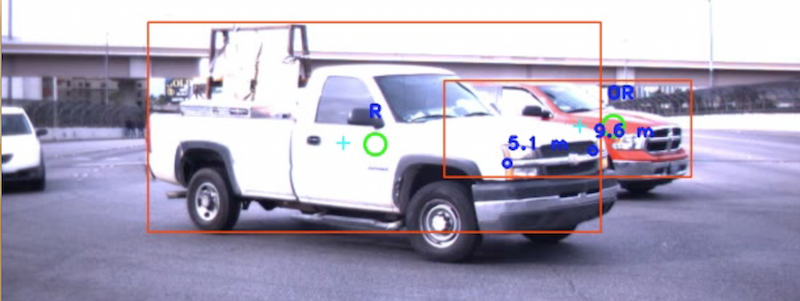
\includegraphics[width=0.4\textwidth]{text/figures/lefttrun2cars.png}
  \captionof{figure}{Partially occluded vehicle detected in a left turn.}
  \label{systemOverview::occludedVehicleDetected}
\end{figure}

\begin{figure}[H]
  \centering
  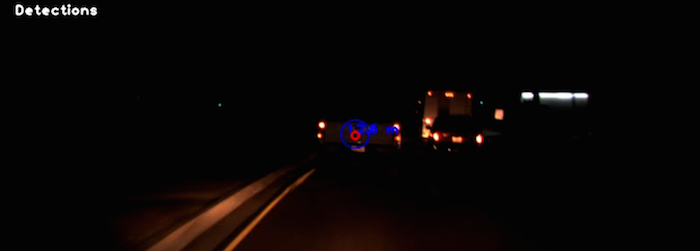
\includegraphics[width=0.4\textwidth]{text/figures/distanceCarEvent.png}
  \captionof{figure}{Distance to vehicle in front of ego-vehicle.}
  \label{systemOverview::distanceToVehicle}
\end{figure}
\end{multicols}
\vspace*{1pt}